\section{Насколько задания были сложными?}

Участникам олимпиады, в рамках заполнения онлайн-опроса (см. Раздел 1 для получения профиля респондентов) было предложено оценить сложность олимпиады по 5-бальной шкале.

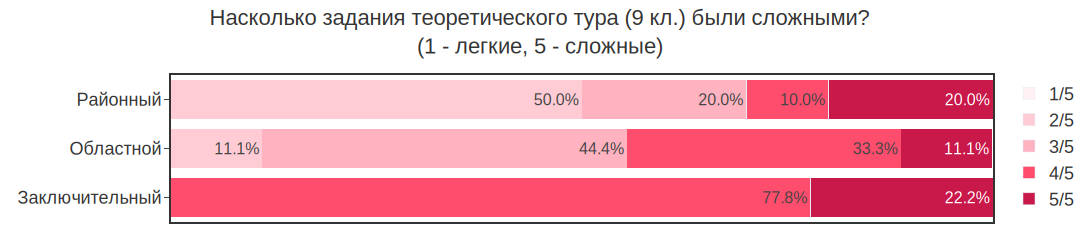
\includegraphics[width=\linewidth]{../export/pdf/demographics/difficulty-grade9.pdf}

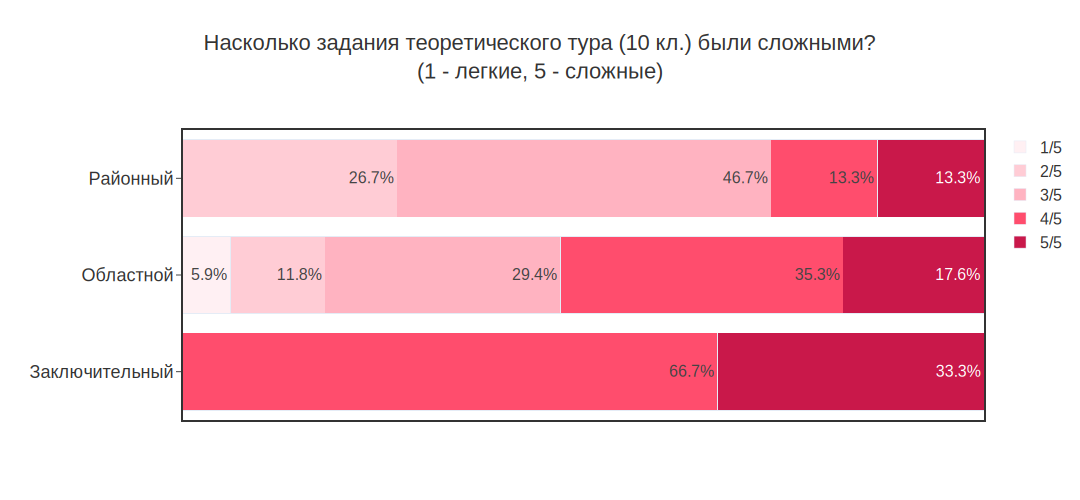
\includegraphics[width=\linewidth]{../export/pdf/demographics/difficulty-grade10.pdf}

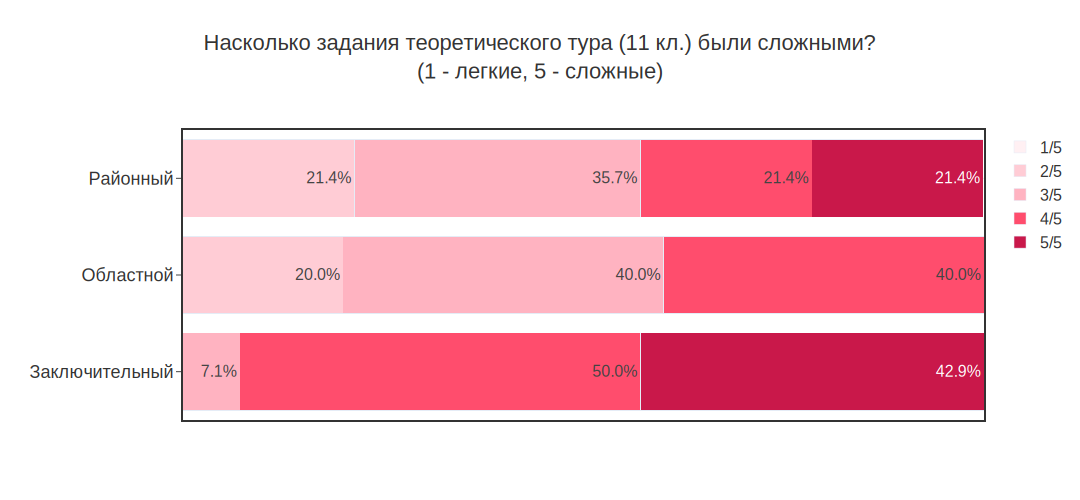
\includegraphics[width=\linewidth]{../export/pdf/demographics/difficulty-grade11.pdf}

\newpage
\section{Насколько задания были объемными?}

Участникам олимпиады предлагалось оценить насколько задания были объемными по 5-бальной шкале.

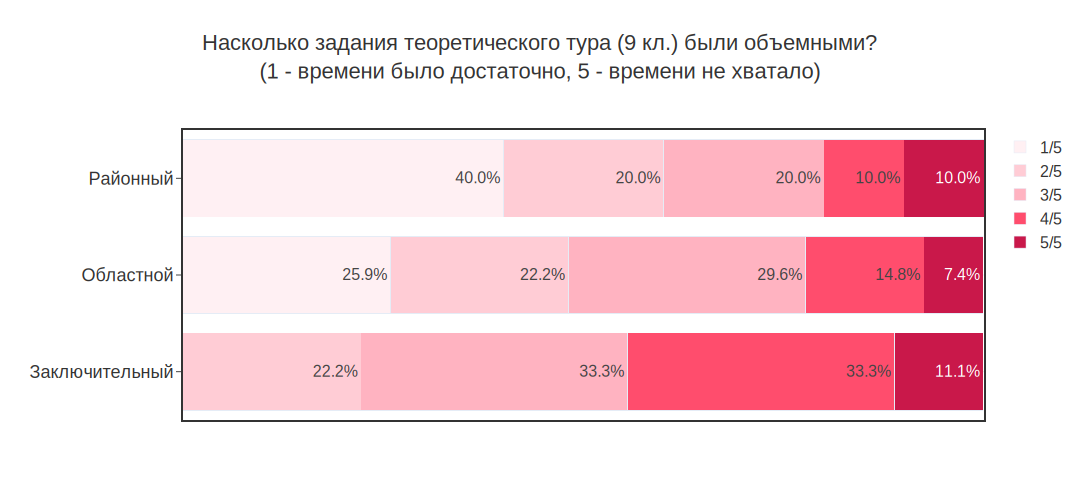
\includegraphics[width=\linewidth]{../export/pdf/demographics/volume-grade9.pdf}

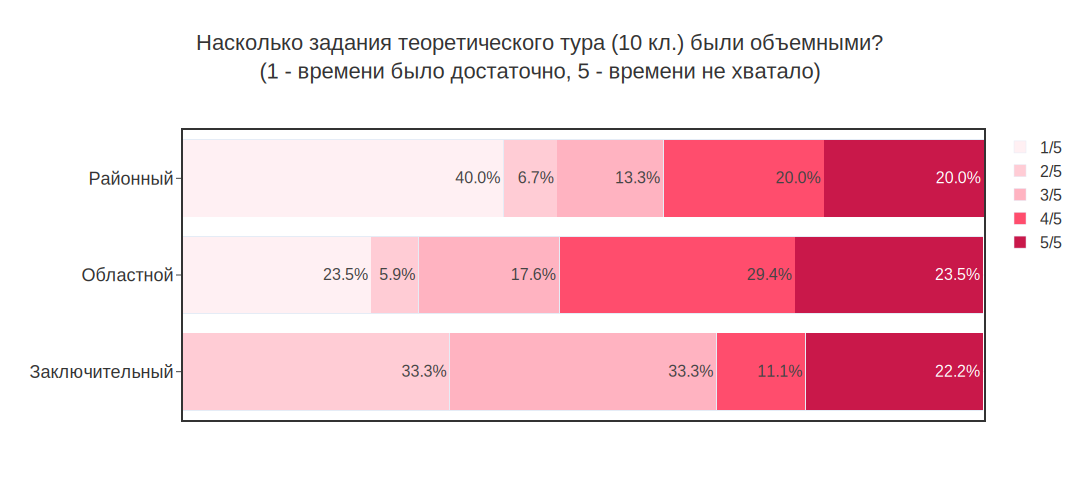
\includegraphics[width=\linewidth]{../export/pdf/demographics/volume-grade10.pdf}

\includegraphics[width=\linewidth]{../export/pdf/demographics/volume-grade11.pdf}

\newpage 

\section{Насколько задания были интересными?}

Участникам олимпиады предлагалось оценить насколько задания были интересными по 5-бальной шкале.

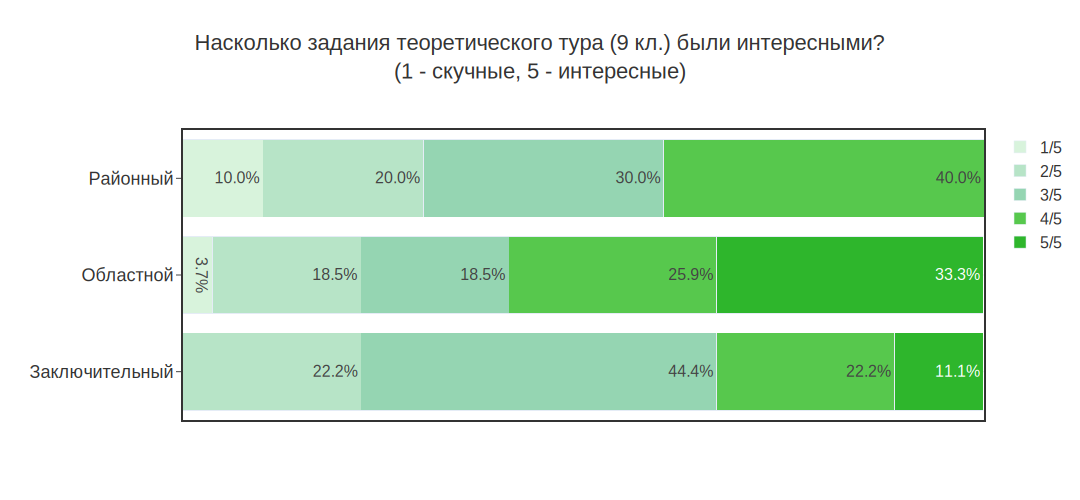
\includegraphics[width=\linewidth]{../export/pdf/demographics/interest-grade9.pdf}

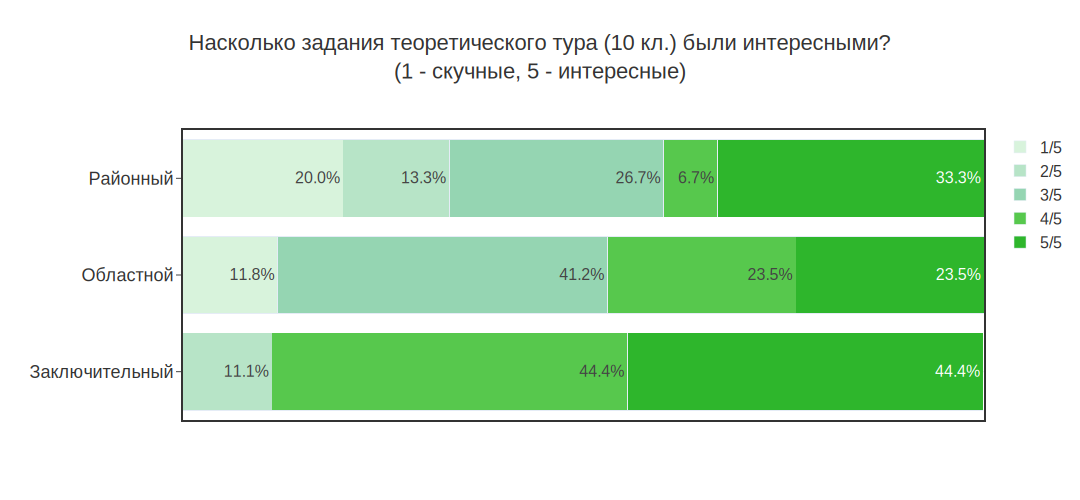
\includegraphics[width=\linewidth]{../export/pdf/demographics/interest-grade10.pdf}

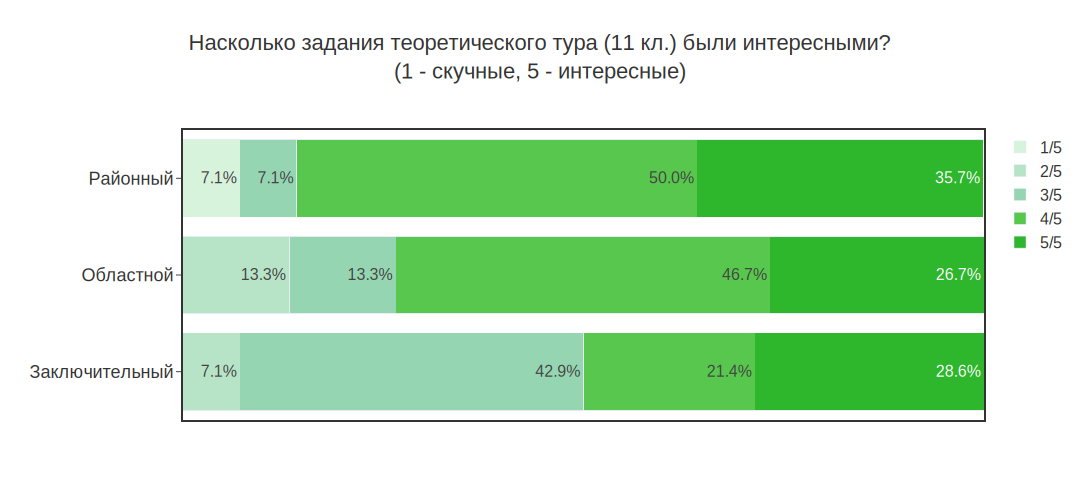
\includegraphics[width=\linewidth]{../export/pdf/demographics/interest-grade11.pdf}


\subsection{Впечатления о районном этапе}
Ученикам предлагалость ответить на следующий вопрос в открытой форме: \textit{Ваши общие впечатления от заданий районной олимпиады? Что понравилось, что не понравилось? Что хотели бы изменить? Скажите все, что считаете нужным сказать.} Орфография и пунктуация респондентов сохранены.

\begin{itemize}
    \itemsep-0.2em
    \item[--] Удивился, так как было легче чем ожидал и чем было на прошлых годах, не понравилось что было задание с титрованием (про кристаллогидрат сульфата никеля)
    \item[--] Жүргіздім. Негізі олимпиада мен мектеп программасыңдағы есептердің деңгейі мүлде сәйкес келмиді. Олимпиада есептері мектеп програмассымен қатар жүргізсе деген өтінішім бар. Себебі олимпиада есептері анағұрлым күрделі.
    \item[--] Думаю все было хорошо продумано. Сложенсть задачек соответствовало уровню районки и по времени все было нормально.
    \item[--] [хотелось бы] усложнить задания, добавить общую химию и глубокие знания неорганической. (\textit{Примечание:} этот отзыв оставлен учеником неспециализированной школы)
    \item[--] Все было отлично
    \item[--] Все хорошо, кроме одного момента, хотелось побольше творчества в заданиях, там например порисовать структуры или применения химии в реальной жизни, с которой мы каждый день сталкиваемся. Ещё не хватило наверное классической для олимпиад органической цепочки или задачи на органику.  
    \item[--] Маған барлығы ұнады, бірақ тапсырмалардың логикасын ұғу қиын болды
    \item[--] Олимпиада была интересной, как и способ подачи материала, в некоторых задачах была излишняя информация, типа задачи \#3, а где-то наоборот, моих знаний не хватило для решения задач. Также не хватило времени, хотя и в аудитории я дописывал один, но думаю другие просто и не пытались. В целом это район мне понравился гораздо больше чем предыдущий, в особенности понравилась последняя задача, думаю задачи на термодинамики с прикладными примерами интересные. \*На задачу \#2 времени просто не хватило , даже не приступил
    \item[--] Мен үшін өте қиын болды
    \item[--] Было немножко трудно, но задание были интересные
    \item[--] Региональные задания были немного проще, чем предыдущие олимпиадные задания, и задания были интересными
    \item[--] Мне было очень интересно
    \item[--] Понравилось : Интересные задачи - Задачи 3, 5 были крайне интересными/интересными соответственно. Полезные задачи - В задаче 4 полезные рассуждения и выводы. То же касается и последнего пункта задачи 5 Не понравилось : Не хватает органики. В прошлом году на районном этапе, была отличная задача на органику (10кл, 5 задача). Чтобы сохранить объем олимпиады, можно было бы заменить органику на задачу 1
    \item[--] Очень интересная олимпиада, только задачи мне кажется легче чем прошлогодние
    \item[--] мне абсолютно все понравилось, все задачи интересные, аж за каждое хваталась. большое спасибо коллегии, за то что они трудятся и за ежегодные авторские задачи.
    \item[--] Задачи были легкими, но думаю так и надо т.к это только районный этап, понравилась 2 задача, сильно напоминает стиль всероссов, хотя щелкается за 5 минут если найдешь азот. В целом задачи довольно легкие решил все примерно за 20-30 минут.
    \item[--] Было достаточно сложно чем я ожидала
\end{itemize}

\subsection{Впечатления об областном этапе}
Ученикам предлагалость ответить на следующий вопрос в открытой форме: \textit{Ваши общие впечатления от заданий областной олимпиады? Что понравилось, что не понравилось? Что хотели бы изменить? Скажите все, что считаете нужным сказать.} Орфография и пунктуация респондентов сохранены.

\begin{itemize}
    \itemsep-0.2em
    \item[--] Задания в довольно часто повторяют идеи районки, но на более высоком уровне, как и идеи на респе в предыдущем году. Последняя задача и задача про серу с галогеном 11 класса показалась гробом в начале решения, но когда находится точка, с который стоит начать, задача упрощается в $10^4$ раз. Понравилось, что давали формулу и константы когда это нужно было, это уравнивает шансы участников и помогает оценить критическое мышление, нежели зубрёшку
    \item[--] Задания видно было классные, но моих знаний на них не хватило 
    \item[--] Задания проще, чем в прошлые годы. Вторая задача интересная
    \item[--] Не понравилось - не было органики
    \item[--] Организация подкачала, а задания интересные,мне понравились
    \item[--] Задачи были довольно скучными и легкими. Надо читать внимательно и все вышло бы(мне кажется)
    \item[--] Думаю в этом году они легче чем в прошлом году. Задачи были интересные
    \item[--] Угадайки были интересными и в меру сложными. Термодинамика(4 задача) была скучная. Электрохимия была интересная и сложнаватая, но объёмная. Органика довольно интересная, но сложная.
    \item[--] Было сложно
    \item[--] Мне очень нравится формат задач. Они были в меру сложными и интересными. Я думаю эти задачи явно повысили мой уровень в их понимании и решении. Формат 3 маленькие и 3 большие задачи очень уместен для организации отведенного времени и увеличения интереса участников олимпиады!
    \item[--] Мне в целом все понравилось, понимаю, куда нужно расти. Задачи интересные, решаемые и заставляющие подумать. Спасибо нашей прекрасной коллегии химиков 
    \item[--] Были нудноваты, прям не было интереса их решать, сухие условия, задача про Мадияра была вначале интерестна, но тоже в какойто момент стала нудной, хоть и довольно много времени уделял решению, вдвое больше чем могло бы понадобиться задаче, всеравно почти уложился в данное время, не было напряжения под конец, а в том что не решил некоторые задачи, виной моя халатность при подготовке.
    \item[--] общие впечатления - надо было больше готовиться. а если серьезно, то в какой-то степени даже обрадовалась, что пришли решабельные задачи. единственное, что не изменилось с прошлой области, так это органика. вечно оставляю ее на потом из за сложности и нехватки времени.
    \item[--] Мне понравились все задачи, хотел поблагодарить коллегию за эту олимпиаду
    \item[--] Задания были довольно интересными по содержанию, но задания 5,6 сложноваты. Можно было бы сделать чуть легче
    \item[--] Именно к составлению задач не имею претензий. А на место проведения есть много вопросов.
    \item[--] Задачи было сложными и интересными
    \item[--] Задания были значительно легкими по сравнению с прошлыми годами. Решабельные задачи. Не понравилось, что потеряла 30 минут из-за низкого подключения сети к вайфай на олимпиаде. А это время мне никто не вернул.
    \item[--] Интересные задания, было легче решать чем в прошлом году. А органика была посложнее
    \item[--] Есть и легкие и трудные задачи, но как по мне для хорошего олимпиадщика не составило бы проблем набрать как минимум 40 из 70.
    \item[--] Задания довольно таки интересные, однако в виду незнания по каким разделам необходимо готовиться , было сложно. Было бы не плохо если бы задания были более менее для уровня средних школ и гимназий, хоть я и являюсь учеником гимназии , однако у нас нет такого времени и возможности, чтобы посвящать себя полностью олимпиаде, так как по всем остальным предметам пишем Сор и Соч, а после обеда есть дополнительные занятия кружкового характера, и наши учителя также не всегда свободны, чтобы дополнительно на нас переключать свое внимание, как достаточно взрослый понимаю их высокую нагрузку. Учителя максимально стараются дать все необходимые знания , однако по вышесказанным причинам , полагаю у них нет возможности всецело посвятить себя подготовке к олимпиаде. (надеюсь, что все учителя такие как в нашей 40 гимназии, стараются максимально нас направить и подготовить к олимпиадам, а также качественно проводить уроки)
    \item[--] самая худшая областная честно
    \item[--] Весьма скучная, но и долгая, прикольных задач не видел
    \item[--] БОЛЬШОЙ РАХМЕТ ЗА ЗАДАЧИ
    \item[--] В целом впечатление от олимпиады хорошее. Не считая однообразных вычислений в 4 задаче, все задачи были интересными. Понравилось более нестандартная (как мне показалось) формулировка пунктов по аналитике во второй задаче
    \item[--] Честно говоря в этом году задания для меня показались легче. Потому что до этого я сидела и минутами не могла понять что просит от меня задача. А в этом году начиная с первого по пятые задачи (кроме органики и второй задачи про неизвестные вещества) были очень даже доступными. чтобы получить максимальные баллы. Лично у меня траблы были с частью где нужно выводить реакции и тд. Потому что по этой части у меня совсем мало опыта, и за это у меня отнимали баллы. А по математической части мне все понравилось.
    \item[--] На мой взгляд, задания 1 тура надо разделить и часть оставить на 2 тур , так как время , данное на 1 тур, слишком маленькое ( 4 часа ,хотя должно минимум 6 часов) , в то время как 2 тур выполняется за 30-40 минут. ( макс. 1 час) Насчет заданий, мне хотелось бы узнать, из каких источников вы берете материал для составления задач, так как я считаю что задания были слишком сложными ( соответствуют 2-3 курсу университета, и нужно максимально сконцентрироваться на изучение химии, чтобы получить хорошие баллы, что это довольно трудно для меня как современного подростка) Спасибо за понимание!
    \item[--] Мне понравились все задачи, они более логичные чем теоретические
\end{itemize}

\subsection{Впечатления о заключительном этапе}
Ученикам предлагалость ответить на следующий вопрос в открытой форме: \textit{Ваши общие впечатления от заданий республиканской олимпиады? Что понравилось, что не понравилось? Что хотели бы изменить? Скажите все, что считаете нужным сказать.}. Орфография и пунктуация респондентов сохранены.

\begin{itemize}
    \itemsep-0.2em
    \item[--] В целом впечатления о комплекте заданий очень положительные, видно что жюри постарались сделать задания как можно более интересными. Темы заданий были достаточно разнообразными. Единственное, что мне не понравилось, это неявность пунктов в задачах Блиц Физхимика и Намешали. Не увидев в пунктах задачи требования обосновать свой ответ, я посчитал ненужным предоставлять обоснования к своим ответам, особенно учитывая, что пункты задач были сформулированы как закрытые вопросы. Думаю, многие учащиеся, включая меня, предоставили более развернутые ответы на вопросы, если бы это требование было прописано более очевидно в условии задач. Помимо этого, мне показалось, что возможно марк схема по данным задачам была черезчур придирчивой, но с другой стоионы, я понимаю, что ученик предоставивший более полное и правильное обоснование в своем ответе звслуживает больше баллов. Тем не менее, я остаюсь при своем мнении о неочевидности требования предоставить обоснования к своим ответам в этих задачах.
    \item[--] Мне очень сильно понравились задачи на физхимию (4 и 5), в которых надо было использовать логику и мат. аппарат. Эти задания, особенно пятая, довольно близки к самой науке, что сподвигло меня кликнуть и прочитать прикрепленные научные статьи. Именно такие задачи, на мой взгляд, пробуждают интерес у учеников не только к химии, но к науке в целом. Скорее всего единственный минус таких задач в том, что на апелляции выстраивается очередь до 50 человек даже после 4 часов. Это скорее к организации, но думаю есть способ сделать ответы неоспоримыми и однозначными. Смотря на задачи, я понимаю какой это большой труд делать такую работу, но меня все еще не покидает мысль, что их можно как-то улучшить, добавить какие то детали, сделать более интересными и запоминающимися. Буду продолжать думать насчет этого...
    \item[--] Задания хорошие, но чувствуется колоссальное различие в сложностью с задачами прошлых лет на респе. Задачи заставляли задуматься в ином ракурсе нежели другие химические задачи, что кому-то понравилось, а кому-то нет, лично мне понравилось, ведь оценивает как кругозор, так и умение мыслить.
    \item[--] Задания составлялись больше на знание хорошей математичкского аппарата нежели что то химияеское или логичное. Последнее задание казалось особо нелогичным, а 7ое буквально не давало шанса на хороший балл без зубрежки (допустим) Алексеева. Лично мне больше всех понравилась 2ая задача (про кобальт) и 4ая более менее на логику.
    \item[--] Задачи не сбалансированы, 6 неорганик и 1 физхимия. Не лучше ли было сделать 4 неорганики, 1 органику, 1 физхимию и 1 аналитику. Баллы не сбалансированы, за расчеты которые занимали пол страницы могли дать столько же, а иногда и меньше баллов чем за какую-то одну реакцию. Были задачи в которых стоит тебе ошибиться лишь в 1 реакций, то за задачу сразу 0, несмотря на то, что идей и многое другое почти идентично с правильным решением. 
    \item[--] Имхо, в этом году ты должен был, именно знать некоторые вещи. Реакций с кровяной солью, электролиз оксалата, и тп. Если честно прошлые года (2019-2022) были намного легче для меня (набирал 80\%). Я жутко занервничал и написал плохо. Хотелось бы, чтобы в задачах нужно было меньше знать и можно было вывести все самому.
    \item[--] Думаю надо включать задачи с разных тем химии. Аналитика, физхимия, общая химияи тд. Прикольно было то что участников проверяли с разных областей. По типу математики, анализирующей точки, на мировоззрение.
    \item[--] Очень понравились переплетение математики и физики на олимпиаде то есть не только знание химии нужны чтобы решить нужно иметь хоть какие то знание по математике. Не понравилось то что задачи были очень громозкими для всех. Все получили маленькие по отношению общему числу баллов
    \item[--] Задания были интересными, но вторая задача у 11 класса с комплексами (хорошо, что не моими) была тяжёлой, кто ее решал тот не успел решить остальное
    \item[--] Вроде все нормально, т.к это была моя первая офф олимпиада было огромное давление, и не смог написать на свой максимум(как и все).
    \item[--] Если учитывать, что это респа, то справедливо. Я готовился к респе по прошлым годам, и этот год был крайне другой. И стиль задач будто изменился колоссально(если просто посчитать средний балл прошлого и этого года на 1 туре). 
    \item[--] Задания были в некоторых моментах не продуманы до конца в плане деталей, ведь диапазон ответов был широким и несколько вариантов ответа были возможны. Более того, задания были существенно труднее среднестатистического уровня сложности республиканских олимпиад.
    \item[--] Мне кажется, задачи были слишком объемными; 5 часов с учетом стресса не хватало никак. Одна задача занимала 3 страницы, на чтение условии ушло полчаса. В целом, формат с прошлой респы слишком сильно изменился (не говорю, что это плохо, но желательно видеть плавный переход). Две из 8 задач были сделаны в стиле Всероссийской, к чему никто не был готов. В этом году, честно, разочаровалась в задачах, тк многие описания были на знания, нежели на понимание концепта. В прошлых годах можно было решить парочку задач с помощью логики, вчитываясь в условия задач, однако в этому году логика видимо не проверялась.
    \item[--] Очень тяжелые и непонятные,или я просто плохо знаю химию
    \item[--] думаю каждый писал об этом - задачи гроб, но, наверное, это из-за упавшего уровня знаний учеников. Задачи по сравнению с прошлым годом вводят в дизмораль с первых минут, но они необычные и очень интересные. Так как я не готовился к Олимпиаде, не могу сполна оценить их, но сделав вывод со слов других учащихся - думаю стоило бы добавить подсказок. Понравились задачи, но не понравилась их сложность. После олимпиады меня переполняли чувства заинтересованности (в науке), усталости и сильнейшего разочорования в себе) Составителям печенек
    \item[--] Слишком много неорганики, мало физ хим. и не было аналитики. Не было много тем с силлабуса.
    \item[--] Задачи конечно не легкие,но скучные. Понравилась последняя задача только и 6 была интересная, но за нее по нулям скорее всего. Надеялась еа аналитику и органику, не было в итоге ничего
    \item[--] слишком много баллов за легкие задачи, зачем они вообще на респе, 4-7 классные
    \item[--] Республиканская олимпиада была сложнее предыдущих по моим ощущениям. Возможно, из-за подготовки я часто смотрел решения и считал ее легкой, однако эти задания что-то с чем-то. Особенно 6 задача (9кл) на монетку. Слишком мало информации, как по мне. 7 задачу не стоит винить в сложности. Пункт с BF3 и сродством к электрону для меня совсем новая, было бы интересно решить, если бы не усталость и нехватка времени. Впринципе, олимпа норм как для уровня респы. Но организация хромает.
\end{itemize}